\documentclass[10pt,table]{article}
\usepackage[dvipsnames]{xcolor}
%\usepackage{hyperref}
%\usepackage{amsmath}
\usepackage{tikz}
\usepackage{qtree}
\usepackage{tikz-qtree}
%\usepackage{pgfplots}
\usepackage{listings}
%\definecolor{light-gray}{gray}{0.95}
\usepackage{listings}
\usepackage{setspace}
\renewcommand{\baselinestretch}{1.3} 
\usepackage{graphicx}
\usepackage[export]{adjustbox}
\usepackage{amsmath,amssymb,amsthm,amsfonts,amssymb}
\usepackage{fancyhdr}
\usepackage[b4paper]{geometry}
\usepackage{enumitem}
\usepackage{algorithm}
\usepackage{algpseudocode}
\usepackage{multicol}
\setlength\columnsep{30pt}
\usepackage{setspace}



\setlength{\parindent}{0pt}
\setlength{\parskip}{5pt plus 1pt}
\setlength{\headheight}{13.6pt}
\newcommand\question[1]{\vspace{1.2em}\hrule\textbf{ #1}\vspace{.5em}\hrule}
\renewcommand\part[1]{\vspace{.10in}\textbf{#1)} \enspace}
\pagestyle{fancyplain}
\fancyhf{}
\renewcommand{\headrulewidth}{1.4pt}
\lhead{\textbf{\ANDREWID }}
\cfoot{\textbf{First Draft } - \thepage   }
\rhead{\rule[-1ex]{0pt}{3.5ex} Hossein Naderi }
\newcommand\ANDREWID{Trying to explain the algorithm in simple language} 
\newcommand\HWNUM{1}
\newtheorem{theorem}{Theorem}
\newtheorem{lemma}[theorem]{Lemma}
\theoremstyle{definition}
\newtheorem{definition}{Definition}
\algnewcommand\algorithmicforeach{\textbf{for each}}
\algdef{S}[FOR]{ForEach}[1]{\algorithmicforeach\ #1\ \algorithmicdo}

\begin{document}

\question{Previous Work}

\begin{table}[hbt]
  \begin{center}
  \begin{tabular}{l|c|c|c|c|c}
    & Type & Progress Property & Conditions & Amortized Time Complexity & Space \\
    \hline
    & & & & & \\
  \end{tabular}
  \caption{}
  \end{center}
\end{table}


\question{Goal}
The model consists of $p$ processes. And the problem is to implement linearizable shared queue Q supporting $<ENQ, DEQ>$ operations between them.

%
%\begin{figure}[h]
%\begin{center}
%\tikzset{every picture/.style={line width=0.75pt}} %set default line width to 0.75pt        
%
%\begin{tikzpicture}[x=0.75pt,y=0.75pt,yscale=-1,xscale=1]
%%uncomment if require: \path (0,300); %set diagram left start at 0, and has height of 300
%
%%Curve Lines [id:da24404451870478872] 
%\draw    (102,43) .. controls (143.58,47.95) and (138.12,104.85) .. (199.13,107.92) ;
%\draw [shift={(201,108)}, rotate = 181.82] [color={rgb, 255:red, 0; green, 0; blue, 0 }  ][line width=0.75]    (10.93,-3.29) .. controls (6.95,-1.4) and (3.31,-0.3) .. (0,0) .. controls (3.31,0.3) and (6.95,1.4) .. (10.93,3.29)   ;
%%Curve Lines [id:da9272135872377072] 
%\draw    (102,121) .. controls (141.6,91.3) and (162.58,119.43) .. (224.12,117.08) ;
%\draw [shift={(226,117)}, rotate = 537.27] [color={rgb, 255:red, 0; green, 0; blue, 0 }  ][line width=0.75]    (10.93,-3.29) .. controls (6.95,-1.4) and (3.31,-0.3) .. (0,0) .. controls (3.31,0.3) and (6.95,1.4) .. (10.93,3.29)   ;
%%Curve Lines [id:da5453903537732101] 
%\draw    (101,182) .. controls (158.42,196.85) and (149.19,136.23) .. (203.34,122.4) ;
%\draw [shift={(205,122)}, rotate = 526.9300000000001] [color={rgb, 255:red, 0; green, 0; blue, 0 }  ][line width=0.75]    (10.93,-3.29) .. controls (6.95,-1.4) and (3.31,-0.3) .. (0,0) .. controls (3.31,0.3) and (6.95,1.4) .. (10.93,3.29)   ;
%%Shape: Grid [id:dp5927814714859243] 
%\draw  [draw opacity=0] (238,105) -- (350,105) -- (350,126) -- (238,126) -- cycle ; \draw   (238,105) -- (238,126)(258,105) -- (258,126)(278,105) -- (278,126)(298,105) -- (298,126)(318,105) -- (318,126)(338,105) -- (338,126) ; \draw   (238,105) -- (350,105)(238,125) -- (350,125) ; \draw    ;
%%Curve Lines [id:da33961815970017184] 
%\draw    (359,115) .. controls (398.6,85.3) and (399,117.35) .. (457.22,115.08) ;
%\draw [shift={(459,115)}, rotate = 537.14] [color={rgb, 255:red, 0; green, 0; blue, 0 }  ][line width=0.75]    (10.93,-3.29) .. controls (6.95,-1.4) and (3.31,-0.3) .. (0,0) .. controls (3.31,0.3) and (6.95,1.4) .. (10.93,3.29)   ;
%%Curve Lines [id:da9041409242658852] 
%\draw    (359,115) .. controls (400.58,104.11) and (400.02,164.77) .. (458.22,160.16) ;
%\draw [shift={(460,160)}, rotate = 534.29] [color={rgb, 255:red, 0; green, 0; blue, 0 }  ][line width=0.75]    (10.93,-3.29) .. controls (6.95,-1.4) and (3.31,-0.3) .. (0,0) .. controls (3.31,0.3) and (6.95,1.4) .. (10.93,3.29)   ;
%%Curve Lines [id:da2855643108836211] 
%\draw    (359,115) .. controls (379.79,51.64) and (412.34,55.91) .. (458.59,71.52) ;
%\draw [shift={(460,72)}, rotate = 198.8] [color={rgb, 255:red, 0; green, 0; blue, 0 }  ][line width=0.75]    (10.93,-3.29) .. controls (6.95,-1.4) and (3.31,-0.3) .. (0,0) .. controls (3.31,0.3) and (6.95,1.4) .. (10.93,3.29)   ;
%
%\end{tikzpicture}
%\caption{Multiple queries on the shared Queue}
%\end{center}
%\end{figure}

%We show operation $o$ requested by process $p$ by $o_p$ and the shared queue by $Q$ and local queues by $q$.

If $op$ finishes before $op^\prime$ starts, it has to take effect on the $Q$ before another. For concurrent operations from processes on $Q$, the implementation can decide which to put before the other. So we want to design an algorithm that gives processes responses and does their operation on the $Q$. Since the linearization is a complete ordering among given operations, our problem is to agree on a linearization of the operations.


\begin{figure}[h]
\begin{center}
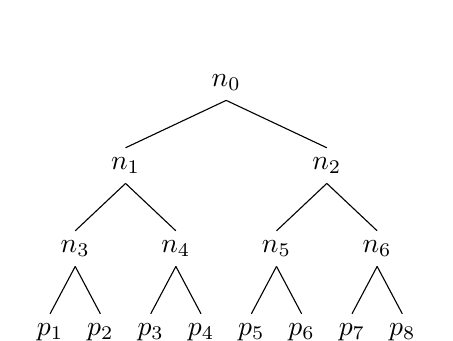
\begin{tikzpicture}
\Tree [.$n_0$ [.$n_1$ [.$n_3$ $p_1$ $p_2$ ] [.$n_4$ $p_3$ $p_4$ ] ]
          [.$n_2$ [.$n_5$ $p_5$ $p_6$ ] [.$n_6$ $p_7$ $p_8$ ] ] ]
\end{tikzpicture}
\caption{The total ordering of all requests operation propagated up to the root is stored in the root. A request it done if it has reached to the root and has been added to the history. In each node we store which requests has been propagated up to it.}
\end{center}
\end{figure}


A usual way \cite{JayantiP05} to agree on something is to use tournament trees. Consider a tournament tree where each process is assigned to one of its leaves. Each process adds an operation to its leaf and tries to propagate it up to the root. The first one that reaches the root is the first operation. Thus the tournament tree is like a competition between processes to determine the total ordering. Propagating an operation from a node means trying to move it one level higher than its parent. Sometimes, two operations from two nodes are propagated up to the parent concurrently; we have to choose one to be before the other arbitrarily.

Now two problems arise:
\begin{itemize}
  \item Since the tournament tree is shared among all the processes, then at some point, there may be multiple processes trying to propagate their operations at the same node. So we need a lock-free procedure for propagating operations from children of a node to it.
  \item One way to implement a shared object with the tournament tree is to store in each node the ordering of operations propagated up to that node. Merging of the two children of the root gives us the total ordering at some point. But keeping all these data is not memory-efficient. For example, all dequeues straight after a queue that gets empty can return null without knowing the whole history before.
\end{itemize} 
\pagebreak
\question{First Try}

In the first attempt, we store each subtree ordering of operation in its root. At each propagation step, we append children's new operations to the parent ordering.  The merging step is heavy, and this way is not memory-efficient. Each ordering merge step is $O(p)$, and there will be $\log(p)$ propagate steps, and it will take $O(\#operations)$ to compute the operation response.

\begin{figure}[h]
\begin{center}
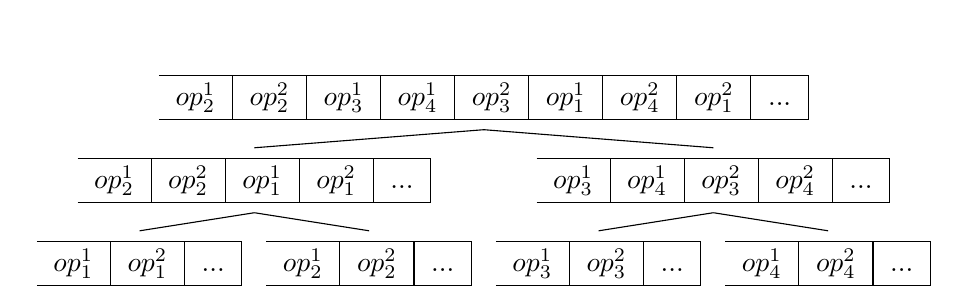
\begin{tikzpicture}
  
\Tree [.{\begin{tabular}{l|c|c|c|c|c|c|c|c|c}  \hline  $op_2^1$ & $op_2^2$ & $op_3^1$ & $op_4^1$ & $op_3^2$ & $op_1^1$ & $op_4^2$ & $op_1^2$ & ... \\ \hline\end{tabular}}  [.{\begin{tabular}{l|c|c|c|c|c}  \hline $op_2^1$ & $op_2^2$ & $op_1^1$ & $op_1^2$ & ... \\ \hline\end{tabular}}
      {\begin{tabular}{l|c|c|c}  \hline $op_1^1$ & $op_1^2$ & ... \\ \hline\end{tabular}} {\begin{tabular}{l|c|c|c}  \hline $op_2^1$ & $op_2^2$ & ... \\ \hline\end{tabular}} ] [.{\begin{tabular}{l|c|c|c|c|c}  \hline $op_3^1$ & $op_4^1$ & $op_3^2$ & $op_4^2$ & ... \\ \hline\end{tabular}} {\begin{tabular}{l|c|c|c}  \hline $op_3^1$ & $op_3^2$ & ... \\ \hline\end{tabular}} {\begin{tabular}{l|c|c|c}  \hline $op_4^1$ & $op_4^2$ & ... \\ \hline\end{tabular}} ] ]

\end{tikzpicture}
\caption{First Try: We show operation $i$ from process $j$ with $op_j^i$. In each node, we store the ordering of all the operations propagated up to it.}
\end{center}
\end{figure}

\begin{algorithm}[h]
\caption{First Try Algorithm}
\begin{algorithmic}[1]

\Procedure{Do}{node n, operation op}
\State n.leaf.append(op)
\State \Call{Propagate}{n}
\State \Return \Call{Compute}{op}
\EndProcedure
\Statex
\Procedure{Propagate}{node n}
\If{r$\neq$root}
\State \Call{MergeChilrenOrderingInto}{n.parent}
\State \Call{Propagate}{r.parent}
\EndIf
\EndProcedure
\Statex
\Procedure{MergeChilrenOrderingInto}{node n}
\State new=n.children.new-operations
\State n.ordering.append(new)
\EndProcedure

\end{algorithmic}
\end{algorithm}

\question{Second Try}

On the first try, we store the ordering of all the operations in the subtree in its root. But it's not necessary for concurrent operations. If two operations are propagated to a node simultaneously, they will be propagated up to the root together so we can store their ordering in the root. This improvement does not change the time complexity of merge steps.

\begin{figure}[h]
\begin{center}
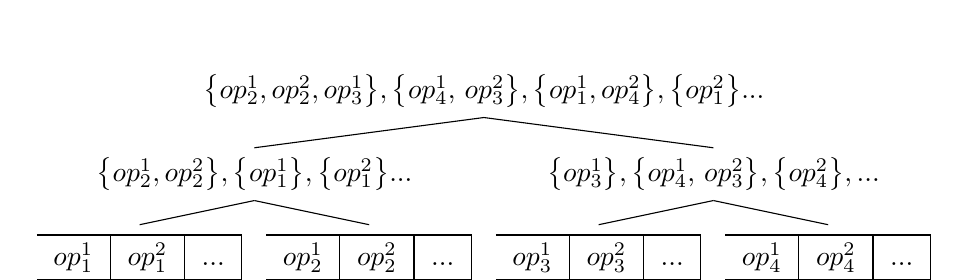
\begin{tikzpicture}
  
\Tree [.{$\big\{op_2^1,op_2^2,op_3^1\big\},\big\{op_4^1$, $op_3^2\big\},\big\{op_1^1, op_4^2\big\},\big\{op_1^2\big\}...$ }  [.{ $\big\{op_2^1, op_2^2\big\},\big\{op_1^1\big\},\big\{op_1^2\big\}...$ }
      {\begin{tabular}{l|c|c|c}  \hline $op_1^1$ & $op_1^2$ & ... \\ \hline\end{tabular}} {\begin{tabular}{l|c|c|c}  \hline $op_2^1$ & $op_2^2$ & ... \\ \hline\end{tabular}} ] [.{ $\big\{op_3^1\big\},\big\{op_4^1$, $op_3^2\big\},\big\{op_4^2\big\},...$ } {\begin{tabular}{l|c|c|c}  \hline $op_3^1$ & $op_3^2$ & ... \\ \hline\end{tabular}} {\begin{tabular}{l|c|c|c} \hline $op_4^1$ & $op_4^2$ & ... \\ \hline\end{tabular}} ] ]

\end{tikzpicture}
\caption{Second Try: In each internal node, we store the set of all the operations propagated together up to it, and one can arbitrarily linearize the total of concurrent operations.}
\end{center}
\end{figure}

\pagebreak
\question{Third Try}

We call sets in the ordering from Algorithm 2 "blocks". Here we are proposing that if you store some constant statistics in each set, you can compute the set. If you know how many operations from the left child and right child are in block b, then with knowing the count of operations before block b in node n, we can find out which operation from each child of n has propagated to block b. This leads us to the main algorithm. Using this approach, we can make merge steps $O(\log p)$. As we said before, if we know some data like what is the size of the queue, it helps us to compute results faster. In this way, we propose our algorithm to compute the dequeue operation in $O(\log^2p)$. 


%\begin{figure}[h]
%\begin{center}
%\begin{tikzpicture}
%  
%\Tree [.{\begin{tabular}{l|c|c|c|c|c|c|c|c|c}  \hline $root$ & $\pi$ & $\chi$ & $\varphi$ & $\Delta$ & $\theta$ & $\Upsilon$ & $\xi$ & $\eta$ & ... \\ \hline\end{tabular}}  [.{\begin{tabular}{l|c|c|c|c}  \hline $n_1$ & $B_{11}$ & $B_{12}$ & $B_{13}$ & ... \\ \hline\end{tabular}}
%      {\begin{tabular}{l|c|c|c}  \hline $p_1$ & $\varphi$ & $\Upsilon$ & ... \\ \hline\end{tabular}} {\begin{tabular}{l|c|c|c}  \hline $p_2$ & $\Delta$ & $\theta$ & ... \\ \hline\end{tabular}} ] [.{\begin{tabular}{l|c|c|c}  \hline $n_2$ & $B_{21}$ & $B_{22}$ & ... \\ \hline\end{tabular}} {\begin{tabular}{l|c|c|c}  \hline $p_3$ & $\chi$ & $\eta$ & ... \\ \hline\end{tabular}} {\begin{tabular}{l|c|c|c}  \hline $p_4$ & $\pi$ & $\xi$ & ... \\ \hline\end{tabular}} ] ]
%
%\end{tikzpicture}
%\caption{Third Try: In each node we store the summary of operation propagated together(some constant size statistics called blocks). Pros: Quick merges and low memory use.}
%\end{center}
%\end{figure}










%If each propagation step is not heavy in our design, then there are at most $\log(p)$ steps. We are trying to implement steps in the nodes $\log(p)$ too. In the remainder, we focus on two parts of the algorithm; the first one deals with the lock-free property of the merge procedure on nodes of the tournament tree, and the second one is about why our design works fast and correctly as a shared queue.
 
 


\question{Merge Step}
In each merge step on node n, we read n.children new operations and try to append them to the n's ordering. Here we propose a wait-free approach using two CAS operations. First, we create a block of newly added operations to n's children(exist in n.children but not in n). After that, we try to append them to the last block; if it wasn't successful, we try again. If one of the $CAS$ operations was successful, then the block is propagated up to the root; otherwise, it means after the first unsuccessful CAS, another operation has come, and it reads current operations.

\texttt{This new algorithm needs proof}

\begin{algorithm}[h]
\caption{Merge Step}
\begin{algorithmic}[1]

\Procedure{MergeChilrenOrderingInto}{node n}

\State block=\Call{CreateBlock}{n.left,n.right}
\State last=n.last \Comment{Index of the first empty cell of n's array of blocks.}
\If{\Call{CAS}{n.last, last, last+1}}
n[last]=block
\ElsIf{\State\Call{CAS}{n.last, last+1, last+2}}
n[last]=block
\EndIf
\EndProcedure

\end{algorithmic}
\end{algorithm}


\question{Data structure details}
Here we are talking about details of the information stored in blocks and the root.

Tree Structure:
\begin{itemize}
  \item Leaf $l$ of the tournamnet tree is the list of the operations of process $p$.
  \item Interval node $n$ stores an array of blocks($n.blocks$) and index of the first empty cell of the array($n.last$).
  \item Root like interval nodes stores blocks with two additional data: size(size of the queue after the block), req($\#$returning deques in each block).
\end{itemize}


In each block we store:
\begin{itemize}
  \item Accumulative $\#$left enqs,$\#$right enqs,$\#$left deqs,$\#$right deqs
  \item pointers to last block merged from left child and righ child
\end{itemize}


How to find the ith enq among all operations? Find the bock containing ith operation in the root using binary search. Decide the operation is in which child and continue recursively.



\texttt{how to draw lists as nodes of the tree and draw edges from cells?}

\begin{center}
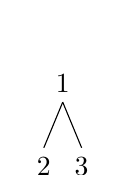
\begin{tikzpicture}

\Tree [.1 2 3 ]

\end{tikzpicture}
\end{center}

And these coloumns in the root:\\

{\begin{tabular}{c|c|c|c|c|c|c|c|c|}
    \hline enq & 5,6 & 5,8 & 6,3 & 3,7 & 10,2 & 1,2 & 2,3 & ... \\
    \hline deq & 3,11 & 3,6 & 5,10 & 7,9 & 3,1 & 2,0 & 9,8 & ... \\
    \hline rdeq & 11 & 9 & 13 & 10 & 4 & 2 & 14 & ... \\ 
    \hline size & 0 & 4 & 0 & 0 & 8 & 9 & 0 &... \\ \hline\end{tabular}}


\question{Complete Algorithm with the Logic related to the Queue}

\begin{algorithm}
\caption{Main Algorithm}\label{alg}
\begin{algorithmic}[1]
\onehalfspacing


\Function{Do}{operation op}
\State add p to this.ops
\State \Call{Propagate}{this.ops}
\State \Comment{When is op added to the root?}
\If{op is a deq}
\State before-size: size of the block before block containing op
\State e: \#enqs in the block containing op
\State d: \#deqs in the block containing op before op
\If{before-size + e - d $<$ 1}
\State \Return{null}
\Else{}
\State d: \#rdeqs before the op in all the ordering
\State \Return{enq(d+1)} \#d+1th enq value in all the enqs
\EndIf
\EndIf
\EndFunction
\Statex

\Function{Propagate}{node n}
\State b=\Call{Create-Block}{n}
\If{!\Call{tryAppend}{b, n}}
\Call{tryAppend}{b, n}
\EndIf
\State \Call{Propagate}{n.parent}
\EndFunction
\Statex

\Function{Create-Block}{n}
\Statex \Comment constructs block of the new operation in children of n. if n is the root, it has extra fields: size, rdeqs.
\EndFunction
\Statex

\Function{tryAppend}{b, n}
\Statex \Comment tries to append b to the last of the n's list.
\EndFunction
\Statex

\Function{Index}{operation op, level $\in$ nodes, type $\in\{$block, operation$\}$}
\Statex \Comment returns index of op in the given level, e.g  Index(op, root, block) return ordering of the block containing op in the root blocks.
\EndFunction
\Statex

\Function{Access}{i, level $\in$ nodes, type $\in\{$enq, deq$\}$}
\Statex \Comment returns i-th operation of given type in the given node subtree.
\EndFunction
\Statex

\Function{Prefix-Sum}{i, level $\in$ nodes, type$\in\{$enq, deq, rdeq$\}$}
\Statex \Comment computes how many of the given type operations are before the ith operation in the given level. For rdeq it will only get root level.
\EndFunction


\end{algorithmic}
\end{algorithm}

\begin{algorithm}
\caption{Block Tree}
\begin{algorithmic}[1]
\begin{multicols}{2}


\Statex $\blacktriangleright$ leaf $l_i$: list of operations
\Statex $\blacktriangleright$ internal node $n$ of BT: list of blocks and index $last$
\Statex $\blacktriangleright$ block $b$: 4 statistics of concurrent operations aggregated together to a block in a \textsc{Refresh} consisting [$left$:$ \#$left ops, $right$: $\#$right ops, $left-sum$: prefix sum left ops, $right-sum$: prefix sum right ops]
\Statex $\blacktriangleright$ index $last$: index of last block of node $n$
\Statex

\Function{void}{Append}{operation op, pid i} 
\State $l_i$.append($op$)
\State \Call{Propagate}{parent of $l_i$}
\EndFunction{Append}

\Statex

\Function{void}{Propagate}{node $n$}
\If{$n$==root} \Return
\Else
\State $new$=\Call{CreateBlock}{n}
\If{\Call{CAS}{$n$.last, now, now+1}}
last block of $n$=now
\ElsIf{\Call{CAS}{$n$.last, now, now+1}}
last block of $n$=now
\EndIf
\EndIf
\State \Call{Propagate}{parent of $n$}
\EndFunction{Propagate}

\Statex

\Function{boolean}{CreateBlock}{node n}
\State $current$= last block of $n$
\State $start$= \Call{BSearch}{crrent.left-sum}
\State $left$=0
\ForEach{$block$}{ $start$: first null block of left child of $n$}
\State $left$+=$block$.left
\EndFor
\State $left-sum$=current.left-sum+left
\State do lines 14 to 19 for right
\State \Return [left,right,left-sum,right-sum]
\EndFunction{CreateBlock}

\columnbreak

\Function{element}{GetIndex}{block b, index i} 
\State n:=b.node
\If{i$\leq$b.left}
\State sb=\Call{BSearch}{left child of $n$, i-b.right.sum}
\State \Call{GetIndex}{sb, b.left-sum} 
\Else ~sb=\Call{ BSearch}{right child of $n$, i-b.left.sum}
\State \Call{GetIndex}{sb, b.right-sum} \EndIf
\EndFunction{GetIndex}

\Statex

\Function{list}{GetElements}{block b} 
\ForEach{block \textbf{in} \Call{GetSubBlocks}{b}}
\State result.append(\Call{GetElements}{})
\EndFor
\State \Return result
\EndFunction{GetElements}

\Statex

\Function{list}{GetSubBlocks}{b}
\State n:=b.node
\State b[-1]=b's previous block
\ForEach{direction \{left, right\}}
\State init=\Call{BSearch}{n.direction, b[-1].direction}
\State end=\Call{BSearch}{n.direction, b.direction}
\State result.append([init:end])
\EndFor
\State \Return result
\EndFunction{GetSubBlocks}

\end{multicols}
\end{algorithmic}
\end{algorithm}

\bibliographystyle{plain}
\bibliography{refrences}


\end{document}




